\documentclass[12pt]{article}
\linespread{1.465}
\usepackage{amsmath}
\usepackage{multicol}
\usepackage{graphicx}

%\documentstyle[11pt]{article}

\setlength{\topmargin}{-.5in}
\setlength{\textheight}{9in}
\setlength{\oddsidemargin}{.125in}
\setlength{\textwidth}{6.25in}


\begin{document}

\noindent

\setlength{\parindent}{0cm}


\section*{Project 1 - Matrix Multiplication}
Team 27 \--- David Eckman, Bryce Evans, Batu Inal

\subsection*{Motivation}

Our assignment was to enhance the performance (GFlops/s) of matrix multiplication ($C = AB$ for $M x M$ square matrices) by improving various parameters such as arithmetic intensity, memory access, and cache efficiency.

\subsection*{Methods}

In our analysis for the task, we considered five main modifications: (1) changing the order of loops for matrix multiplication both within and among blocks; (2) changing the block size relative to cache, (3) copying and restructuring matrices in memory, (4) different compiler flags, (5) using the restrict keyword to achieve strong optimizations by the compiler and combinations thereof. We have also included a section where we discuss our failed attempts to achieve better performance.

\subsubsection{Changing the Order of Loops}

The matrix multiplication algorithm that involves blocking using three nested loops to determine the order of updates both within and among blocks. We tested all orderings of the loops for complete verification. For all combinations, we also tried various optimization flags and block sizes, but found these variables to be independent and have no noticeable significance our selection of the best ordering. Graph 1.1 shows the performance of the ordering which we found to be the most effective at increasing flop rate: k-j-i for both the outer and inner sets of loops. This was an increase of over 100\% over the worst case ordering of k-j-i for both loops, as shown in Graph 1.1.

\begin{center}
\includegraphics[width16cm]{•}

\end{center}
Graph 1.1: Gflops/s vs Dimension for various loop orders


Given the matrices are in column major order and we are optimizing on reducing cache thrashing, it is important that we keep the columns in memory for as long as possible. This includes using a column entirely while in memory and not needing to reload it later. The update formula $C[j*lda+i] \mathrel{+}= A[k*lda+i] * B[j*lda+k] (c_{i,j} \mathrel{+}= a_{i,k} * b_{kj})$ illustrates how the order of the indices affect the access patterns. By putting \texttt{i} in the innermost loop, we fix element $i,j$ of \texttt{B} and pass through column $j$ of $C$ and column $k$ of $A$. This access pattern is the most favorable because of the column major alignment in memory. When $j$ is in the innermost loop, we would fix the $i,k$ element of $A$ and pass through row $i$ of $C$ and row $k$ of $B$. This would be the least desirable access pattern.

Note: While we found very little performance difference between $k$, $j$, $i$, and $j$, $k$, $i$, the former was slightly faster and we have not yet determined why. While theoretically index $j$ should be on the outer most loop because it controls column changes the most, our hypothesis is that the cache is not large enough to keep two entire columns and so these columns are occasionally lost from cache and require a reload.   

\subsubsection{Compiler Flags}

We tried an array of compiler flags for optimizing code. We focused strictly on performance (as opposed to code size, compilation time, or memory usage), using flags that traded these for faster code execution.

\begin{multicols}{3}
\begin{verbatim}
-O3 
-fast 
-opt-prefetch 
-unroll-aggressive
-parallel 
-ansi-alias 
-ftree-vectorize 
-xHost 
-axCORE-AVX2 
\end{verbatim}
\end{multicols}


\texttt{-O3} adds significant optimizations across the board, taking more compile time but interchanging order of operations for improved speeds as well as some loop unrolling (also assisted by \texttt{-unroll-aggressive}). Given our application uses many floating point operations in loops, this is a strong option to increase speed. Using \texttt{-O3} in another application could potentially slow down code execution.

Matrix multiplication does a similar operation many times across many data. We use prefetching to load data into memory without halting execution. We had these ideas suggested to us from gh:\texttt{kenlimmj}.

The remainder of the flags (\texttt{-parallel, -ansi-alias, -ftree-vectorize, -xHost,
-axCORE-AVX2}) include series of options to utilize AVX (Advanced Vector Extensions) and SIMD operations (Single Instruction, Multiple Data).  These add vectorization operations are able to use a single core to load two doubles side by side for processing. Ignoring overhead, this allows to potentially achieve twice the performance without such operations. 

\subsubsection{Restrict Keyword}

The restrict keyword allows for strong optimizations by the compiler. By using restrict, we promise that pointers will be unique and only accessed directly. This allows optimization by not having to reload values repeatedly  after updates. Consider the case of pointer $A $being loaded and it being added to a value at pointer $B$ and pointer $C$. Without using restrict, $A$ would need to be reloaded after updating $B$ because $A$ and $B$ could be the same value.  With restrict, we only load $A$ once, which is appropriate for our usage because we can provide this guarantee as no value in a matrix is ever used to update itself. 


\subsubsection{Block Size Relative to Cache Size}

For the second method, our approach was to partition the matrices into smaller square matrices (blocks) and multiply them. By using this approach we aimed to improve our arithmetic intensity by performing many multiplication operations with the same data. We also aimed to improve our memory access patterns by choosing the block size so that a block each from matrices $A$, $B$, and $C$ could fit into our L1 or L2 cache.

\begin{center}
\includegraphics[width16cm]{•}

Diagram 2.1: Matrix multiplication instantiated from smaller blocks.
\end{center}


On the compute nodes of the totient cluster, L1 cache was 32KB 8-way set-associative, L2 cache was 256 KB 8-way set-associative and L3 was 15MB (shared) 20-way set-associative. Our initial approach was to utilize the L1 cache without regarding the L2 or the L3 cache. Our calculations for the block size required in order to fit three blocks into L1 cache was as follows:

\begin{align*}
32KB * 1024B/KB * 1 double/8B &= 4096 doubles\\
4096 doubles / 3 matrices &\approx 1365 doubles/matrix
\end{align*}
Since there are $N^2$ values in a matrix: \[\sqrt{1365}\approx 36 (Block Size)\]



We predicted that the overhead of going to the L2 cache if there was a miss in L1 cache would be very low. Therefore we made the exact same calculations for fitting three blocks in the L2 cache. The calculated block size was 104 and the resulting performance is shown in Plot 2.1.

As it can be observed from Plot 2.1, we have significant improvement in performance from a median of roughly 3.7 GFlops/s to around 4.2 GFlops/s. We knew that there would be a huge overhead in going from L2 cache to L3 cache but still wanted to test out a bigger block size; to see whether theory matched practice. For the sake of testing we tested a block size of 128. As it is also depicted from Plot 2.1, there was loss in performance in the dimension range of 200-400 as the size of the block was increased, which could be accounted by an increase in cache misses at L1 and L2.


\begin{center}
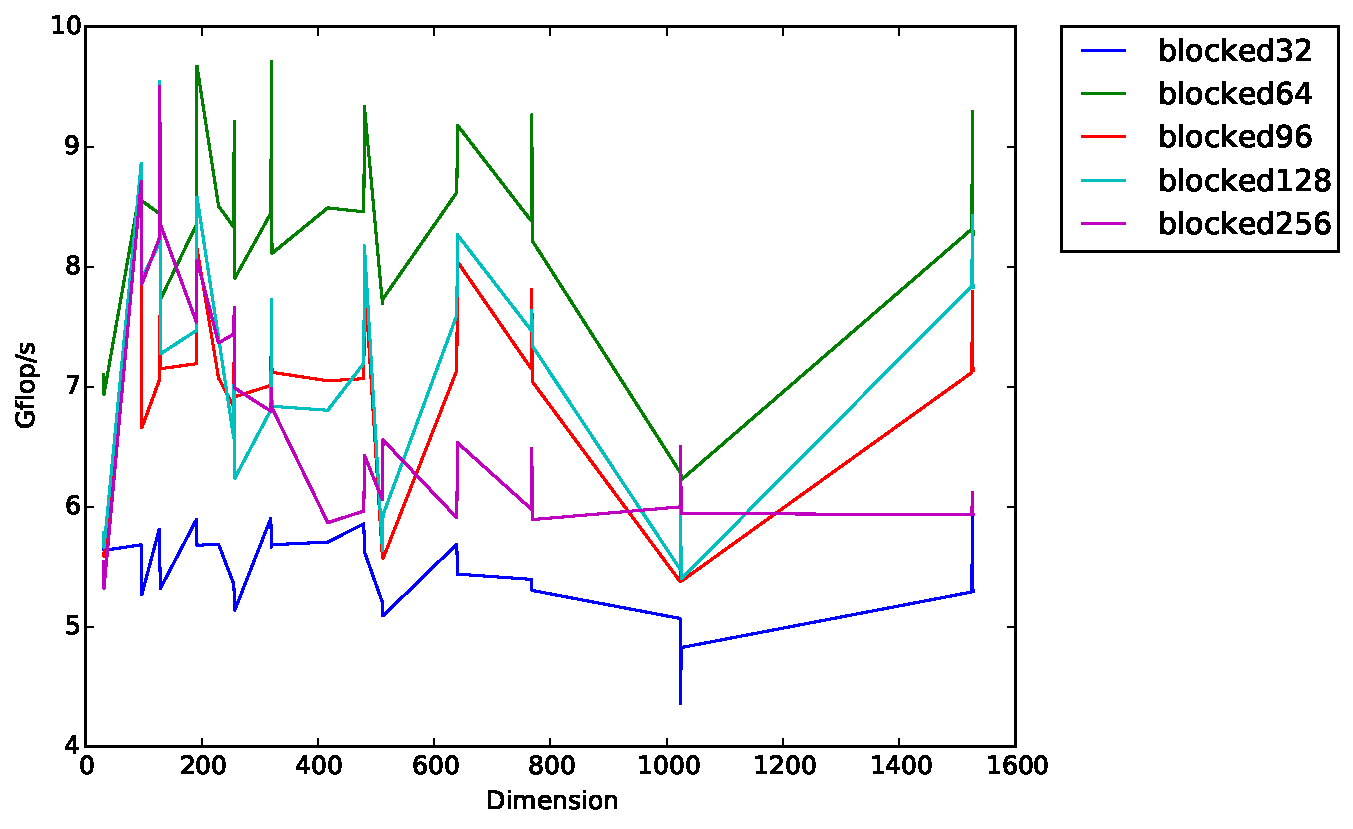
\includegraphics[width=16cm]{timing_blocked_comparison.pdf}

Plot 2.1 Performance for various block sizes
\end{center}


\subsubsection{Copy and Restructure the Matrices in Memory}

Another method we attempted was to copy the matrices A and $B$ matrices into memory to improve memory access patterns during the block multiplication operations. More precisely, we restructured the two matrices so that the elements of each block were stored in contiguous memory in column major form. The blocks themselves were then stored in column major form. (It would be great to have a Plotic showing the memory structure. Same can be said about the memory access patterns for the loop orders.) We chose column major form within and among the blocks of the new matrices because of the ordering of the loops; with the index i in the inner loop, matrices $C$ and A are accessed vertically. We believed that the improved access patterns in the block-block multiplications would outweigh the computational overhead of copying the matrices. We observed a general trend of improving performance as dimension of the matrices increased. We also tested a range of block sizes to tune the copy optimization implementation. 

Insert timing\_copyblocked\_comparison.pdf. Shows copy optimization at a range of block sizes. Block sizes of 96 and 128 were the best out of those tested.

\begin{center}
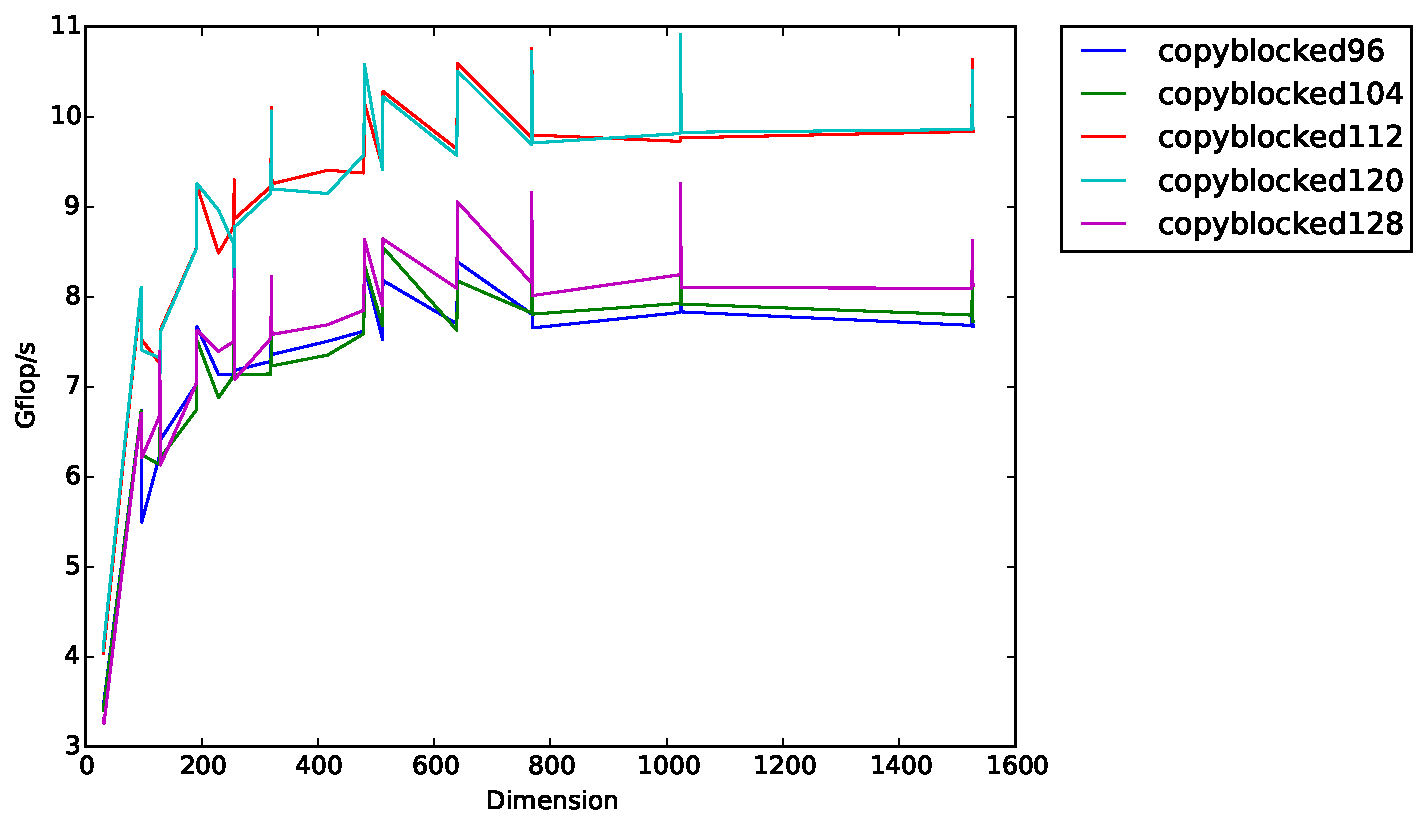
\includegraphics[width=16cm]{timing_copyblocked_comparison_zoom.pdf}

Plot 3.1: Gflops/s vs Dimension for Copying Matrices
\end{center}

Based on the results shown in Plot 3.1, we decided to more closely examine block size between 96 and 128. We chose to test block sizes in this range which were multiples of 8 because that is the number of doubles that fit in a register. From the results in Plot 3.2, we chose the block size of 112 going forward.

Insert timing\_copyblocked\_comparison\_zoom.pdf. Shows copy optimization at a range of block sizes between 96 and 128. 112 and 120 were the best out of those tested.

\begin{center}
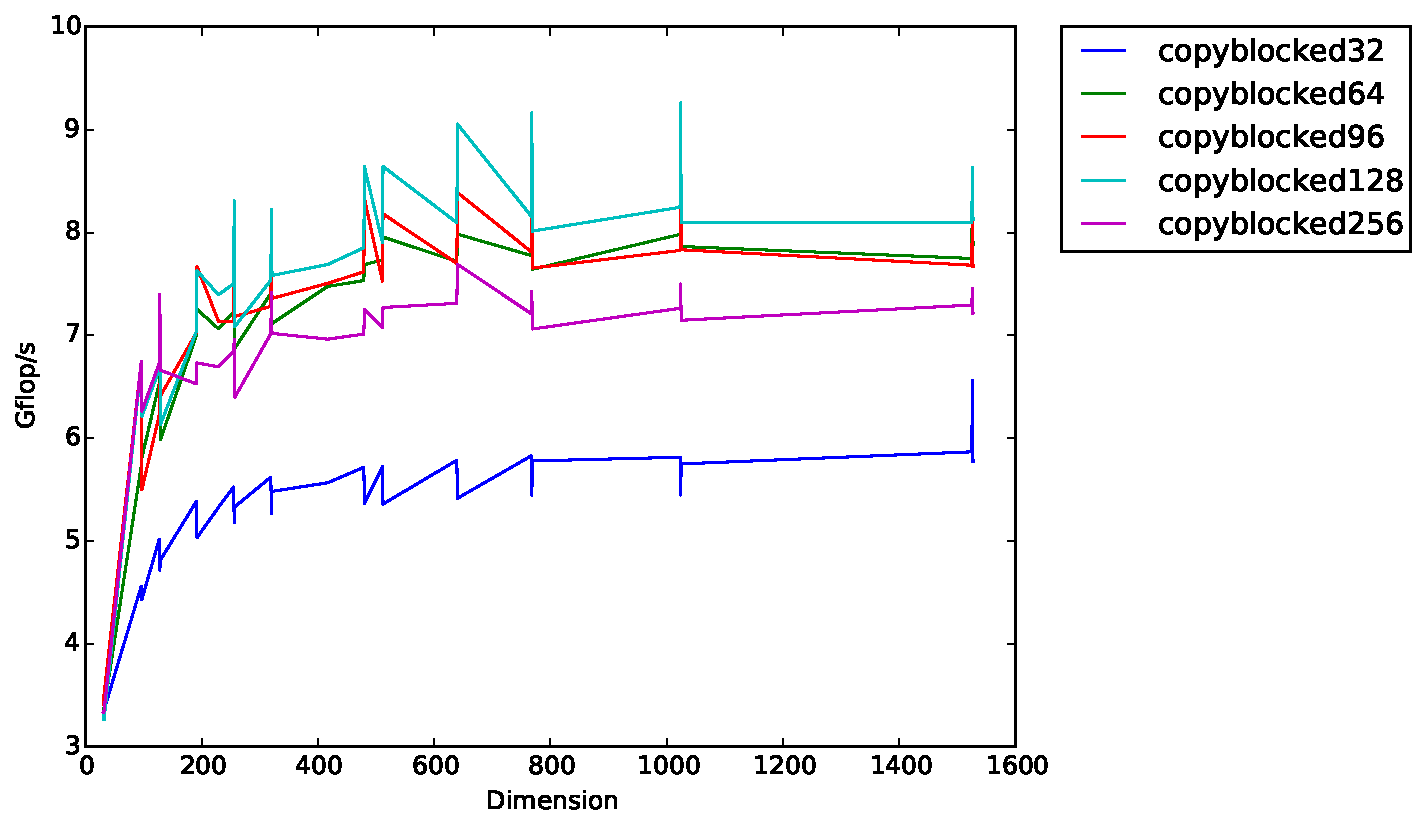
\includegraphics[width=16cm]{timing_copyblocked_comparison.pdf}

Plot 3.2: Gflops/s vs Dimension for Copying Matrices
\end{center}

Lastly, we attempted to perform the copy optimization on the matrix $C$ as well but were unable to fully debug the program. We anticipate that this would have led to further improvements in performance.

Observing our plots, with copying matrices $A$ and $B$, we realized that as copying had a huge overhead, it was not beneficial for small sized matrices. However, the cost of copying was amortized in big matrices, of around $N>200$, thus, proving to enhance performance. We therefore decided to eventually copy the matrices that were over the threshold of 200 and leave them as is, if they were less than the determined threshold of 200.

\subsection{Failed Methods}
We tried a number of methods that did not result in higher performance, namely manual loop unrolling, multi-level blocking, GCC compilation and flags, and a brief attempt to implement sub-cubic multiplication. 

Manual loop unrolling, even across various variables or orders of loops, was not as effective as the compiler unrolling. This was a surprise because other groups in the class (gh: \texttt{sheroze1123}) included this in their implementation and found it to beneficial.  We believe that in our attempts, the compiler no longer optimized these sections despite those optimizations being superior to ours. For multi-level blocking, we copied on each iteration and this overhead surpassed the benefits. Another possibility was we did not optimize for the appropriate cache, choosing to load into L2 and L3, instead of L1 and registers. Given more time, we would attempt this again with better testing of multi-level block sizes to optimize for architecture as well as improved efficiency of copying data. 

With our attempts at gcc compilation, while much more documentation is available for gcc, the vectorization and parallel support was lacking. ICC was far superior with these benefits, giving great performance increases with a few flags and ease of enabling vectorized operations. 

Lastly, we explored alternative methods to do sub-cubic matrix multiplication, but the large overhead and pre-computations were very quickly apparent to dominate the actual time the program would run. If we were to run this program across very large matrices (unable to fit on a single machine, with an order of magnitude more time for computation), this large pre-computation could become advantageous.

\subsection{Summary}

In this paper, we have discussed several approaches towards enhancing the performance (GFlops/s) of matrix multiplication ($C = AB$ for $M \times M$ square matrices) by improving various parameters such as arithmetic intensity, memory access, and cache efficiency. Our initial experiments suggests that; changing the loop ordering to j-k-i, utilizing the compiler optimizations such as AVX (Advanced Vector Extensions) and SIMD operations (Single Instruction, Multiple Data), using the restrict keyword to ensure that pointers will be unique and only accessed directly (thus, letting the compiler do optimizations by not having to reload values repeatedly  after updates), utilizing the L1 and L2 caches by determining an optimal block size of 104 and finally copying the matrices $A$ and $B$ matrices into memory, if the size of matrices is greater than 200, to improve memory access patterns; enhanced the performance of the matrix multiplication by almost factor of eight compared to the naive implementation. Given our failed attempts with various techniques; such as, manual loop unrolling, multi-level blocking, gcc compilation and flags, copy optimization on the matrix $C$  and a brief attempt to implement sub-cubic multiplication; further work could be done to debug our failed attempts and try various techniques in current literature such as aligning the memory in order to have more efficient loads into the Cache. 

\subsection{References}

\begin{verbatim}
https://icl.cs.utk.edu/svn/lapack-dev/lapack/trunk/BLAS/SRC/dgemm.f

\end{verbatim}

\end{document}